\section{Logistic Regression}
Classification method

\subsection{Binary Classification}
\begin{itemize}
    \item Decision with 2 possible outcomes
    \item Hail in Lausanne (yes/no)
    \item Master admission (admission / no admission)
    \item Based on different data / entity
\end{itemize}
$y = 1$ implies yes/accepted/admission, $y = 0$ implies no/rejected \\
$P(y = 1, x_1 = 4.5, x_2 = 5, x_3 = 5.5)$\\

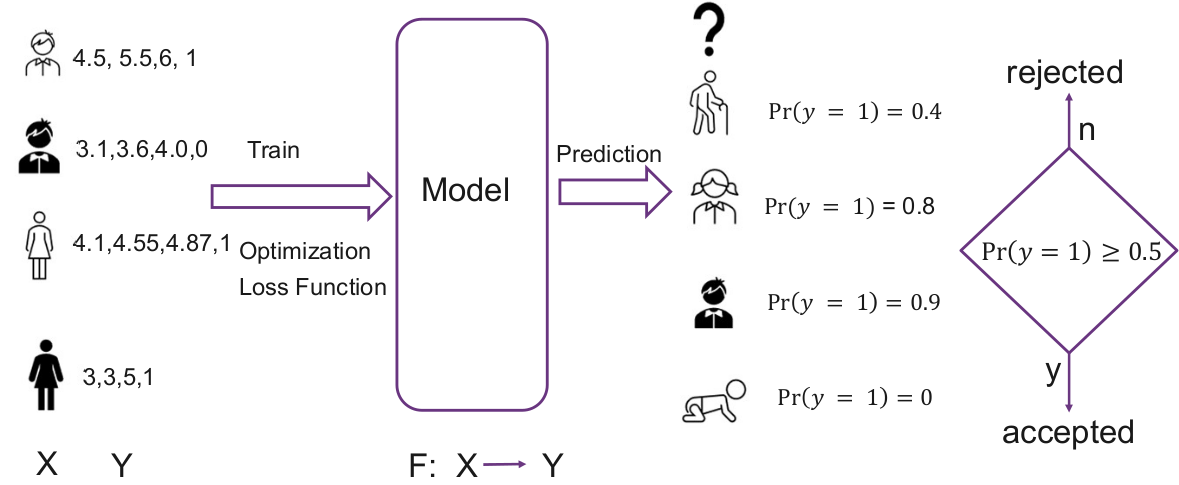
\includegraphics[width=\linewidth]{binary-classification.png}

\subsection{Predicting Probabilities: Logistic Regression}

\textbf{Decision using Linear Regression}
\begin{itemize}
    \item Train the model with gradient descent
    \item \textcolor{blue}{Bad Idea!}
    \item Models the response (y) and post process the response (e.g.\ by thresholding) to compute the probability
\end{itemize}

\textbf{The model: sigmoid function} \\

\begin{itemize}
    \item Values between 0 and 1. $y$ is interpreted as probability
    \item Function is not parametrized
    \item Has a single input value
\end{itemize}

\begin{center}
    $sigmoid(y) = \frac{1}{1 + e^{-y}}$
\end{center}
$y$ is

\begin{itemize}
    \item calculated from the input data
    \item a linear combination of the input features, with one feature $ax_i + b$ with D dimensions $y_i=\sum_{d=0}^{d=D}w_d \cdot x_i^d$
\end{itemize}

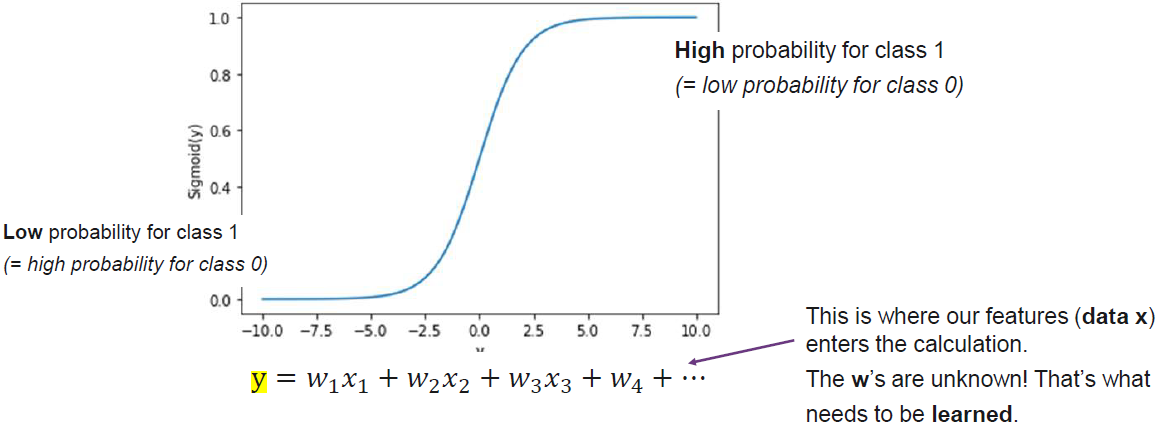
\includegraphics[width=\linewidth]{sigmoid.png}
\textbf{Probabilities}
\begin{itemize}
    \item We can write the estimated probability
    \item For a prediction we can write
\end{itemize}
\begin{center}
    $P(x) = \frac{1}{1 + e^{-(W^{T}x)}}$
\end{center}
\begin{center}
    e.g. $Pr(y_i = 1 | x_i; w) = \Large \frac {1}{1 + e^{-(w_0 + w_1 \cdot x_{i, 1} + w_2 \cdot x_{i, 2} + w_3 \cdot x_{i, 3})}}$
\end{center}
\begin{center}
    Minimize $cost(W) = E = -\frac{1}{N}\sum_{i=1}^N (y_i * log(p_i)) + (1 - y_i) * log(1 - p_i))$
\end{center}

\subsection{Optimization: Maximum Likelihood Estimation}
\begin{itemize}
    \item Given all the data points (X,Y) we want to maximize the probability that all the predictions are correct.
    \item For each of the training data, we want to maximize the likelihood of correct prediction
    \item We can use Gradient Descent to find optimal $W$
\end{itemize}
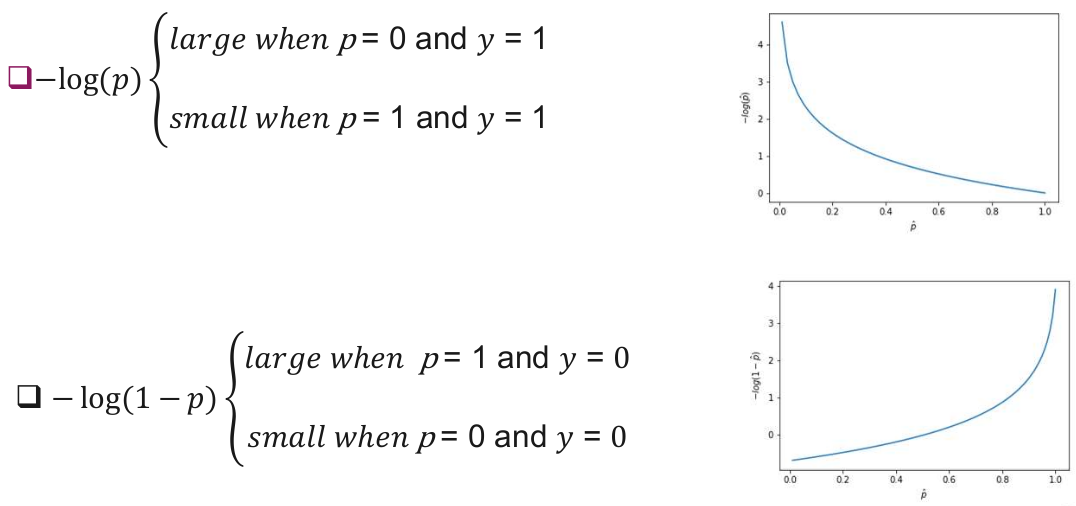
\includegraphics[width=\linewidth]{likelihood-cost.png}

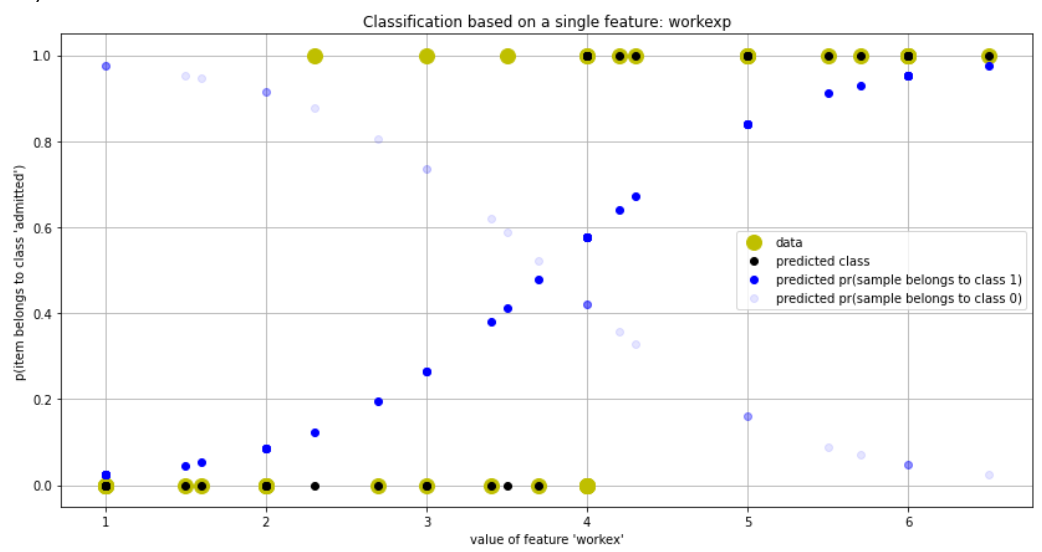
\includegraphics[width=\linewidth]{classification-based-diagram.png}
